\documentclass[journal,12pt,twocolumn]{IEEEtran}

\usepackage{setspace}
\usepackage{gensymb}

\singlespacing 



\usepackage[cmex10]{amsmath}

\usepackage{amsthm}

\usepackage{mathrsfs}
\usepackage{txfonts}
\usepackage{stfloats}
\usepackage{bm}
\usepackage{cite}
\usepackage{cases}
\usepackage{subfig}

\usepackage{longtable}
\usepackage{multirow}

\usepackage{enumitem}
\usepackage{mathtools}
\usepackage{steinmetz}
\usepackage{tikz}
\usepackage{circuitikz}
\usepackage{verbatim}
\usepackage{tfrupee}
\usepackage[breaklinks=true]{hyperref}
\usepackage{graphicx}
\usepackage{tkz-euclide}
\usepackage{float}

\usetikzlibrary{calc,math}
\usepackage{listings}
    \usepackage{color} %%
    \usepackage{array} %%
    \usepackage{longtable} %%
    \usepackage{calc} %%
    \usepackage{multirow} %%
    \usepackage{hhline} %%
    \usepackage{ifthen} %%
    \usepackage{lscape}     
\usepackage{multicol}
\usepackage{chngcntr}
\newcommand{\norm}[1]{\left\lVert#1\right\rVert}

\DeclareMathOperator*{\Res}{Res}

\renewcommand\thesection{\arabic{section}}
\renewcommand\thesubsection{\thesection.\arabic{subsection}}
\renewcommand\thesubsubsection{\thesubsection.\arabic{subsubsection}}

\renewcommand\thesectiondis{\arabic{section}}
\renewcommand\thesubsectiondis{\thesectiondis.\arabic{subsection}}
\renewcommand\thesubsubsectiondis{\thesubsectiondis.\arabic{subsubsection}}


\hyphenation{op-tical net-works semi-conduc-tor}
\def\inputGnumericTable{} %%

\lstset{
%language=C,
frame=single, 
breaklines=true,
columns=fullflexible
}
\begin{document}


\newtheorem{theorem}{Theorem}[section]
\newtheorem{problem}{Problem}
\newtheorem{proposition}{Proposition}[section]
\newtheorem{lemma}{Lemma}[section]
\newtheorem{corollary}[theorem]{Corollary}
\newtheorem{example}{Example}[section]
\newtheorem{definition}[problem]{Definition}

\newcommand{\BEQA}{\begin{eqnarray}}
\newcommand{\EEQA}{\end{eqnarray}}
\newcommand{\define}{\stackrel{\triangle}{=}}
\newcommand\hlight[1]{\tikz[overlay, remember picture,baseline=-\the\dimexpr\fontdimen22\textfont2\relax]\node[rectangle,fill=blue!50,rounded corners,fill opacity = 0.2,draw,thick,text opacity =1] {$#1$};}
\bibliographystyle{IEEEtran}
\providecommand{\mbf}{\mathbf}
\providecommand{\pr}[1]{\ensuremath{\Pr\left(#1\right)}}
\providecommand{\qfunc}[1]{\ensuremath{Q\left(#1\right)}}
\providecommand{\sbrak}[1]{\ensuremath{{}\left[#1\right]}}
\providecommand{\lsbrak}[1]{\ensuremath{{}\left[#1\right.}}
\providecommand{\rsbrak}[1]{\ensuremath{{}\left.#1\right]}}
\providecommand{\brak}[1]{\ensuremath{\left(#1\right)}}
\providecommand{\lbrak}[1]{\ensuremath{\left(#1\right.}}
\providecommand{\rbrak}[1]{\ensuremath{\left.#1\right)}}
\providecommand{\cbrak}[1]{\ensuremath{\left\{#1\right\}}}
\providecommand{\lcbrak}[1]{\ensuremath{\left\{#1\right.}}
\providecommand{\rcbrak}[1]{\ensuremath{\left.#1\right\}}}
\theoremstyle{remark}
\newtheorem{rem}{Remark}
\newcommand{\sgn}{\mathop{\mathrm{sgn}}}
%\providecommand{\abs}[1]{\left\vert#1\right\vert}
\providecommand{\res}[1]{\Res\displaylimits_{#1}} 
\providecommand{\norm}[1]{$\left\lVert#1\right\rVert$}
%\providecommand{\norm}[1]{\lVert#1\rVert}
\providecommand{\mtx}[1]{\mathbf{#1}}
%\providecommand{\mean}[1]{E\left[ #1 \right]}
\providecommand{\fourier}{\overset{\mathcal{F}}{ \rightleftharpoons}}
%\providecommand{\hilbert}{\overset{\mathcal{H}}{ \rightleftharpoons}}
\providecommand{\system}{\overset{\mathcal{H}}{ \longleftrightarrow}}
 %\newcommand{\solution}[2]{\textbf{Solution:}{#1}}
\newcommand{\solution}{\noindent \textbf{Solution: }}
\newcommand{\cosec}{\,\text{cosec}\,}
\providecommand{\dec}[2]{\ensuremath{\overset{#1}{\underset{#2}{\gtrless}}}}
\newcommand{\myvec}[1]{\ensuremath{\begin{pmatrix}#1\end{pmatrix}}}
\newcommand{\mydet}[1]{\ensuremath{\begin{vmatrix}#1\end{vmatrix}}}
\numberwithin{equation}{subsection}
\makeatletter
\@addtoreset{figure}{problem}
\makeatother
\let\StandardTheFigure\thefigure
\let\vec\mathbf
\renewcommand{\thefigure}{\theproblem}
\def\putbox#1#2#3{\makebox[0in][l]{\makebox[#1][l]{}\raisebox{\baselineskip}[0in][0in]{\raisebox{#2}[0in][0in]{#3}}}}
     \def\rightbox#1{\makebox[0in][r]{#1}}
     \def\centbox#1{\makebox[0in]{#1}}
     \def\topbox#1{\raisebox{-\baselineskip}[0in][0in]{#1}}
     \def\midbox#1{\raisebox{-0.5\baselineskip}[0in][0in]{#1}}
\vspace{3cm}
\title{Assignment No.5}
\author{Panisha Gundelli}
\maketitle
\newpage
\bigskip
\renewcommand{\thefigure}{\theenumi}
\renewcommand{\thetable}{\theenumi}
Download latex-tikz codes from
\begin{lstlisting}
https://github.com/Panisha707/ASSIGNMENT05/blob/main/main.tex
\end{lstlisting}
%
Download python codes from
\begin{lstlisting}
https://github.com/Panisha707/ASSIGNMENT05/blob/main/untitled31.py
\end{lstlisting}
%
Question taken from
\begin{lstlisting}
quad_form, exercises 2.24
\end{lstlisting}
\section{Question No 1}
Find the coordinates of the focus, axis, the equation of the directrix and latus rectum of the parabola $y^2 = 8x$
\section{Solution}
Given equation of the parabola is:
\begin{align}
    y^2=8x\\
    y^2-8x=0\\
    y^2+2(-4)=0
\end{align}
comparing it with standard equation
\begin{align}
    ax^2+2bxy+cy^2+2dx+2ey+f=0
\end{align}
$\therefore$  a = b = e = 0, d = -4, c = 1, f = 0
\begin{align}
   \vec{V}=\myvec{a&b\\b&c}=\myvec{0&0\\0&1}\\
   \vec{u}=\myvec{-4\\0} 
\end{align}
\begin{lemma}
The equation of a parabola is:
\begin{align}
    \vec{x}^T\vec{V}\vec{x}+2\vec{u}^T\vec{x}+f=0
\end{align}
Then its vertex can be calculated as :
\begin{align}
    \myvec{\vec{u}^T+\eta\vec{p_1}^T\\\vec{V}}\vec{c}=\myvec{\vec{-f}\\\eta\vec{p_1}-\vec{u}}\\
    \text{where, } \eta=\vec{u^T}\vec{p_1}
\end{align}
\end{lemma}
Equation of the parabola can be written as
\begin{align}
   \implies \myvec{0&0\\0&1}\vec{x}+2\myvec{-4&0}\vec{x}+0=0
\end{align}
We can find the eigen values corresponding to the $\vec{V}$,
\begin{align}
\left|\vec{V}-\lambda\vec{I}\right| =\left|\myvec{0-\lambda&0\\0&1-\lambda}\right|
\end{align}
\begin{align}
    \brak{-\lambda}\brak{1-\lambda}=0
\end{align}
$\therefore$
Eigen values are $ \lambda_1=0,\lambda_2=1$
\\
Calculating the eigen vectors corresponding to  $ \lambda_1=0,\lambda_2=1$ respectively
\begin{align}
    \vec{V}\vec{x}=\lambda\vec{x}
\end{align}
\begin{align}
   \implies \vec{p_1}=\myvec{1\\0}\\
   \implies \vec{p_2}=\myvec{0\\1}
\end{align}
The vertex of the parabola can be given as
\begin{align}
    \myvec{\vec{u}^T+\eta\vec{p_1}^T\\\vec{V}}\vec{c}=\myvec{\vec{-f}\\\eta\vec{p_1}-\vec{u}}\\
   \text{where, } \eta=\vec{u^T}\vec{p_1}=\myvec{-4&0}\myvec{1\\0}
    \end{align}
\begin{align}
    \myvec{-8&1\\0&0\\0&1}\vec{c}=\myvec{0\\0\\0}\\
    \implies \vec{c}=\myvec{0\\0}
\end{align}
Since $\lambda_2 > \lambda_1$\\
Hence, the axis using $\vec{p_2}$ is given by
\begin{align}
    \vec{p_2}^T\myvec{\vec{x}-\vec{c}}=0
    \end{align}
    \begin{align}
     \myvec{0&1}\myvec{x\\y}=0   
    \end{align}
    \begin{align}
       \implies y=0 
    \end{align}
    \begin{align}
    \myvec{0&1}\vec{x}=0
\end{align}
\begin{theorem}
The eccentricity, directrices and foci of parabola are given by\\ 
\text{Eccentricity,}
\begin{align}
    e&= \sqrt{1-\frac{\lambda_1}{\lambda_2}} \label{eq:1}
\end{align}
\begin{align}
  \vec{n}&= \sqrt{\lambda_2}\vec{p}_1 \label{eq:2}
  \end{align}
  \begin{align}
  c = \frac{\norm{\vec{u}}^2 - \lambda_2 f   }{2e^2\vec{u}^{\top}\vec{n}} \label{eq:3}
  \end{align}
 \text{Focus,} 
 \begin{align}
  \vec{F}  &= \frac{ce^2\vec{n}-\vec{u}}{\lambda_2}\label{eq:4}
\end{align}
\text{Directrix,}
\begin{align}
\vec{n}^T \vec{x}=c \label{eq:5}
 \end{align}
\end{theorem}
From Equation \ref{eq:1}, eccentricity can be calculated as
\begin{align}
    e&= \sqrt{1-\frac{\lambda_1}{\lambda_2}}
\end{align}
\begin{align}
    e&= \sqrt{1-\frac{0}{1}} =\sqrt{1}\\
     \implies e&= 1
\end{align}
Substituting $\lambda_2$ and $\vec{p_1}$ values in Equation {\ref{eq:2}}
\begin{align}
   \vec{n}&= \sqrt{\lambda_2}\vec{p}_1\\
   \vec{n}&= \sqrt{1}\myvec{1\\0}\\
   \implies \vec{n}&=\myvec{1\\0}
\end{align}
Equation \ref{eq:3} can be calculated as
\begin{align}
    c = \frac{\norm{\vec{u}}^2 - \lambda_2 f   }{2e^2\vec{u}^{\top}\vec{n}}
\end{align}
\begin{align}
    c = \frac{16-1\times0}{2 \times 1^2 \times \myvec{-4&0}\myvec{1\\0}}
\end{align}
\begin{align}
    =\frac{16}{-8}\\
    \implies c = -2
\end{align}
Focus of the parabolic equation can be calculated from the equation \ref{eq:4} 
 \begin{align}
  \vec{F}  &= \frac{ce^2\vec{n}-\vec{u}}{\lambda_2}
\end{align}
 \begin{align}
  \vec{F}  &= \frac{-2 \times 1 \times \myvec{1\\0}-\myvec{-4\\0}}{1}
\end{align}
\begin{align}
   \implies \vec{F}=\myvec{2\\0} 
\end{align}
Directrix of the parabolic equation can be calculated from equation \ref{eq:5}
\begin{align}
   \vec{n}^T \vec{x}=c 
\end{align}
\begin{align}
    \myvec{1&0}\vec{x}=-2
\end{align}
Latus rectum is the line which is parallel to the directrix, passes through the focus and four times of the focal length. Since, the focal length of the parabola is 2.\\
$\therefore$ Latus rectum is 8
\numberwithin{figure}{section}
\begin{figure}[ht]
    \centering
    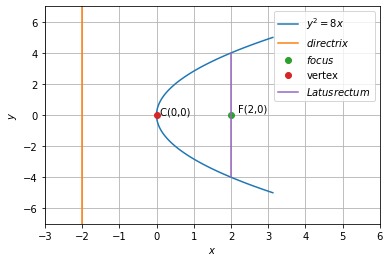
\includegraphics[width=\columnwidth]{parabola.png}
    \caption{Parabola}
    \label{Graphical solution}
\end{figure}
\end{document}
